\iffalse
	前言:
		参考自一个祖传的模板,以及https://github.com/LeyuDame/BNUCV/tree/main 上的BNU的latex简历模板中的代码。
		注意要用XeLaTeX编译链进行编译,且要进行三次编译才能显示照片。问就是LaTeX的锅。
		vscode+latex的话,配置的json中"latex-workshop.latex.recipes"添加:
		{
            "name": "XeLaTeX*3",
            "tools": [
                "xelatex",
                "xelatex",
                "xelatex"
            ]
        }
		即可使用三次XeLaTeX编译。

		LaTeX+VScode怎么配置看https://www.zhihu.com/column/p/166523064。

        每个章节的格式都能混着用,顺序都可以变,只是给了个例子。
        比如你找工作,可以把技能那部分往前挪。
        比如你竞赛经历很多,你就往前挪。
        比如你觉得“其他”有点多余,就删了。

        主要贡献还是把原本word的那个模板页眉页脚和背景完美加进来了。
        LaTeX排版就是很整齐,强迫症狂喜。


        然后就是更新之后就不需要手动为每一页添加页脚页眉背景了。但是新建页面/换页要用'\newnewpage'而不是'\newpage'。
        原本想的是用EveryPageHook来自动添加的,但是有一个bug:第一页的背景透明度会失效,变得很丑,就像直接使用background包一样。
        如果有知道怎么简单的,可发布的方法来解决这个bug的话,请github/gitee联系我。

        记得要三次XeLaTeX编译!!!
        记得要三次XeLaTeX编译!!!
        记得要三次XeLaTeX编译!!!
        这个很重要,所以说三遍!
        可以试试两次的,好像某些环境两次编译也能显示图像,但最好还是三次编译。
\fi

\documentclass[11pt]{article}
\usepackage{tikz}
\usetikzlibrary{calc}
\usepackage{xltxtra}
\usepackage{bookmark}
\usepackage{hyperref}
\hypersetup{hidelinks}
\usepackage{url}
\urlstyle{tt}
\usepackage{multicol}
\usepackage{xcolor}
\usepackage{calc}
\usepackage{graphicx}
\usepackage{fontspec}
\usepackage{xeCJK}
\usepackage{relsize}
\usepackage{xspace}
\usepackage{fontawesome}
\usepackage{titlesec}
\usepackage{enumitem}
\usepackage{siunitx}
\usepackage{amssymb}
\usepackage{tabularx}
\usepackage{multicol}
\usepackage{fontspec}
\usepackage{caption}
\usepackage{everypage}


%%%%%%%%%%%%%%%%%%%%%%%%%%%%%%%%%%%%%%%%%%%%%%%%%%%%%%%%%%%%%%%%%
%							记得改这里							%
%%%%%%%%%%%%%%%%%%%%%%%%%%%%%%%%%%%%%%%%%%%%%%%%%%%%%%%%%%%%%%%%% 
% 学院
\newcommand{\configSchool}{电子信息学院 | School of Electronics And Information}
% 也可以不写英语
%\newcommand{\school}{电子信息学院}
% 联系方式
\newcommand{\configContact}
{
    %\small              % 换了更小的字号
    %\footnotesize       % 这比上面的小一号
    \scriptsize         % 这比上面的再小一号
    \textcolor{white}
    {
        \faEnvelope \quad \href{mailto:xxxx@mail.nwpu.edu.cn}{xxxx@mail.nwpu.edu.cn}    % 邮箱,前面的超链接可以直达邮箱软件
        \hspace{4em}    % 这里可以调间距
        \faWechat \quad xxxxxxxxxxxxx               % 微信
        \hspace{4em}    % 这里可以调间距
        \faPhone \quad 12345678900                  % 手机号
        \hspace{4em}    % 这里可以调间距
        \faGithub \quad \href{https://github.com/xxxx}{https://github.com/xxxx}         % github
    }
}

%%%%%%%%%%%%%%%%%%%%%%%%%%%%%%%%%%%%%%%%%%%%%%%%%%%%%%%%%%%%%%%%%
%							页面设置							%
%%%%%%%%%%%%%%%%%%%%%%%%%%%%%%%%%%%%%%%%%%%%%%%%%%%%%%%%%%%%%%%%% 
% 页面大小与页边距,按需求调整
\usepackage[
	a4paper,
	left=1.2cm,
	right=1.2cm,
	top=1cm,
	bottom=1.5cm,
	nohead
]{geometry}
\newcommand{\newnewpage}{
    \newpage
    背景
	\begin{tikzpicture}[remember picture, overlay]
        % 背景
		\node[opacity=0.05](background) at(current page.center){
			
\includegraphics[width=0.7\paperwidth, keepaspectratio]{images/npu_logo_big.png}
		};
        % 页眉
        \node[anchor=north, inner sep=0pt](header) at (current page.north){
			
\includegraphics[width=\paperwidth]{images/header.png}
		};
        % 校徽
		\node[anchor=west](school_logo) at (header.west){
			\hspace{0.5cm}
			
\includegraphics[width=0.25\textwidth]{images/npu_logo_2.png}
		};
        % 学院名
		\node[anchor=east](school_name) at(header.east){
			\textcolor{white}{\textbf{\configSchool}}
			\hspace{0.5cm}
		};
        % 页脚
        \node[anchor=south, inner sep=0pt](footer) at (current page.south){
			
\includegraphics[width=\paperwidth]{images/footer.png}
		};
        % 联系方式
        \node[anchor=center] at(footer.center){\configContact};
	\end{tikzpicture}
}

%%%%%%%%%%%%%%%%%%%%%%%%%%%%%%%%%%%%%%%%%%%%%%%%%%%%%%%%%%%%%%%%%
%							字体设置							%
%%%%%%%%%%%%%%%%%%%%%%%%%%%%%%%%%%%%%%%%%%%%%%%%%%%%%%%%%%%%%%%%% 
% 英文字体
\setmainfont[
    Path=fonts/,
    Extension=.ttf,
    BoldFont=* Bold,
]{Microsoft Yahei}
% 中文字体
\setCJKmainfont[
    Path=fonts/,
    Extension=.ttf,
    BoldFont=* Bold,
]{Microsoft Yahei}

%%%%%%%%%%%%%%%%%%%%%%%%%%%%%%%%%%%%%%%%%%%%%%%%%%%%%%%%%%%%%%%%%
%							样式设置							%
%%%%%%%%%%%%%%%%%%%%%%%%%%%%%%%%%%%%%%%%%%%%%%%%%%%%%%%%%%%%%%%%%
% 一级标题
\titleformat{\section}					    % 将原标题前面的数字取消了
  {\LARGE\bfseries\raggedright} 		    % 字体改为LARGE,bold,左对齐
  {}{0em}                      			    % 可用于添加全局标题前缀
  {}                           			    % 可用于添加代码
  [{\color{NPU_Blue}\titlerule}]            % 标题下方加一条线
\titlespacing*{\section}{0cm}{*1.2}{*1.5}	% 标题左边留白,上方1.2倍,下方1.2倍

% 二级标题
\titleformat{\subsection}				    % 将原二级标题前面的数字取消了
  {\large\bfseries\raggedright} 		    % 字体改为large,bold,左对齐
  {}{0em}                      			    % 可用于添加全局二级标题前缀
  {}                           			    % 可用于添加代码
  []
\titlespacing*{\subsection}{0cm}{*1.2}{*1.5}% 二级标题左边留白,上方1.2倍,下方1.2倍

% 图例的caption格式设置
\captionsetup[figure]{
    labelfont={},
    labelformat={default},
    labelsep=period,name={图}               % 这里表示你的caption会以“图1”,“图2”,“图3”开头,可以自行更换前缀
}

\CJKsetecglue{}							            % 取消中文字符与数字之间的间隔
\setlength{\parindent}{0pt}							% 取消全局段落缩进
\pagenumbering{gobble}								% 取消页码显示

% 这是个更好看的C++写法,你直接写C++的话,+号会很大,可以使用\Cpp来代替
\protected\def\Cpp{{C\nolinebreak[4]\hspace{-.05em}\raisebox{.28ex}{\relsize{-1}++}}\xspace}
% 中文字符间距
\renewcommand{\CJKglue}{\hskip 0.05em}
% 这里把表格的行间距调成1.2倍了
\renewcommand{\arraystretch}{1.2}
% 这里把正文的行间距调成1.2倍了
\linespread{1.2}

% 主题色
% 西工大蓝
\definecolor{NPU_Blue}{RGB}{0, 80, 158}

%%%%%%%%%%%%%%%%%%%%%%%%%%%%%%%%%%%%%%%%%%%%%%%%%%%%%%%%%%%%%%%%%
%							正文开始							%
%%%%%%%%%%%%%%%%%%%%%%%%%%%%%%%%%%%%%%%%%%%%%%%%%%%%%%%%%%%%%%%%%
\begin{document}
    % 新建页面,这个别删
    \newnewpage


	% 个人信息
    \begin{figure}[h]
        % 左半边,信息,比例占行宽87%,可以自己调
        \begin{minipage}{0.87\textwidth}
            \section{\makebox[\widthof{\faUser}][c]{\color{NPU_Blue}{\faUser}}\quad 个人信息}
            \begin{tabularx}{\linewidth}{p{\widthof{出生日期:}}Xp{\widthof{政治面貌:}}X}
                姓名: & 叁叁 & 性别: & 男 \\
                出生日期: & 2003年11月18日 & 政治面貌: & 党员 \\
                    
                %% 想多加几行的话,就按上面的格式自行补充
                %% 想加粗的话\textbf{}
                %% 想多加几列的话,把\begin{tabularx}{\textwidth}{这里}的内容改一下,可以自己搜一下tabularx怎么用,也可以问gpt/文心一言/讯飞。
            \end{tabularx}
        \end{minipage}
        % 右半边,照片,比例占行宽12%,可以自己调
        % images/example_avatar.png 替换成你证件照的路径。
        \begin{minipage}{0.12\textwidth}
            
\includegraphics[width=\linewidth]{images/example_avatar.png}
        \end{minipage}
        % 尽量留至少1%的间距,不然会换行
    \end{figure}
    \vspace{-2em}


	% 教育背景
    	% \faGraduationCap这类\fa开头的都是font awesome里的logo,想换成其他logo的话,可以看一下附带的fontawsome.pdf,自行替换。
		% \section{\makebox[\widthof{     这里!    }][c]{\color{NPU_Blue}{     和这里!    }}\quad 标题}
	\section{\makebox[\widthof{\faGraduationCap}][c]{\color{NPU_Blue}{\faGraduationCap}}\quad 教育背景}
	\vspace{-1em}
    \begin{table}[h!]
        \begin{tabularx}{\textwidth}{XXp{\widthof{2021年 -- 预计2025年7月毕业}}}
            西北工业大学电子信息学院 & 电子信息工程 & 2021年 -- 预计2025年7月毕业\\
            \textbf{GPA: 3.776/4.1} & \textbf{GPA排名: ??/??} & \textbf{综测排名: ??/??} \\
            % 这里哪个高就加粗哪个,哪个不想放就留白 =w= 比如你综测高GPA低,你就只放综测和综测排名就好。
        \end{tabularx}
    \end{table}
    % 已修课程,可以不放,最好还是放点对口的课
    {
        \small
        已修课程:计算方法,机器视觉与人工智能,计算机视觉技术,语音信号处理,智能人机交互与视觉感知综合设计,遥感信息获取与处理导论,通信原理,高频电子线路
    }


    % 项目经历(找导师一般都看中这个),可以改成“科研经历”
        % \faGears 这是齿轮,适合机械类,我电信的也喜欢齿轮,就用这个了
        % \faFlask 这是烧瓶,适合生化类
        % \faLaptop 这是个笔记本电脑,适合计算机类
        % \faUsers 这是三个人,适合商科
        % 小技巧,老师想看的重点加粗,比如商科类的一般更想看到数字,工科类的更想看到技术
    \section{\makebox[\widthof{\faGears}][c]{\color{NPU_Blue}{\faGears}}\quad 项目经历}
    \vspace{0.5em}              % subsection和section之间加一个0.5em会好看点
    \subsection{APTX4869药物研发\hfill 国家级大创-优秀结题}
    
    \textbf{第一负责人} \hfill 2022年7月-2023年7月
    
    主要负责药物的\textbf{前期研发,中期亲自试药和后期的投毒计划部署}与主要执行人员。成功将著名侦探\textbf{工藤新一}变成小孩摸样。药物的研发成功让\textbf{150万人}收益,最终盈利\textbf{3000万元},效果图见图~\ref{fig: example_1}。
    
    % 这是个工科类加粗的例子
    \vspace{1em}                % 这是换行用的
    \subsection{Improving Multi-Modal Brain Tumor Detection with Contrastive Learning and CLIP Prompt Fine-Tuning \hfill EI会议-在投}

    \textbf{学生独作} \hfill 2024年1月-2023年12月
    
    \textbf{(标题与内容由GPT乱编的,现实中应该没有这论文吧。。大概。)}\textbf{独自进行前期研究,实验验证和论文写作}。重点探索了将\textbf{多模态医学影像}(如MRI和CT)与\textbf{自然语言模型}相结合的方法,以提高脑肿瘤检测的准确性。成功将对比学习和Prompt Fine-Tuning技术应用于医学影像分析中,将模型在脑肿瘤检测任务中的性能提升到了\textbf{超越SOTA的水平},特别是在 one-shot 场景下取得了显著的改进。

    % 不知道写啥好
    \vspace{1em}                % 这是换行用的
    \subsection{基于阴间蓝牙通信系统的高速运转机器设计\hfill SCI期刊-二区在投}
        
    \textbf{一作} \hfill 2023年12月-2024年1月
    
    你有这么\textbf{高速运转的机械}进入中国,进入我给出的原理,小时候。就是\textbf{研发人},就是研发这个东西的原理是\textbf{阴间政权}管。你知道为什么有圣灵给它\textbf{运转仙位}?还有专门饲养这个?为什么地下产这种东西?他管的他是五世同堂旗下子孙。你以为我跟你闹着玩儿呢?你不警察吗?黄龙江一带全都\textbf{带蓝牙}。黄龙江我告诉你在阴间是是那个化名,化名我小舅,亲小舅,张学兰的那个嫡子、嫡孙。产品渲染图见图~\ref{fig: example_2}。

    % 在研的也能写
    % 课程大作业也能写,但是不要标明是大作业就行
    % 一个例子,别真写金工实习做榔头
    \vspace{1em}
    \subsection{大国工匠-论锤子是怎么炼成的\hfill 工程项目-已完结}
        
    \textbf{主要技术负责人} \hfill 忘了日期
    
    对古代中国工匠制作锤子的历史、工艺和技术进行深入研究,包括原材料的选择、工具的制作、锤子的设计和锻造工艺等方面。结合现代工艺技术和设计理念,探索如何将古代工匠的技艺与现代制造工艺相结合,以提高锤子的性能、品质和设计。通过实际制作锤子的过程,验证理论和技术的可行性,并对制作过程中的关键环节进行深入分析和总结,成品见图~\ref{fig: example_3}。


    % 换页
    \newnewpage


    % 图例
        % 用minipage可以一行多图,只需控制每张图的宽度就行
        % 0.32\linewidth 表示一张图占行宽32%,每个都预留一点空间,避免溢出换行
        % [b] 表示下对齐。[t]是上对齐,可以自行更改。
    \begin{figure}[h!]
        \centering
        \scriptsize
        \begin{minipage}[b]{0.32\linewidth}
            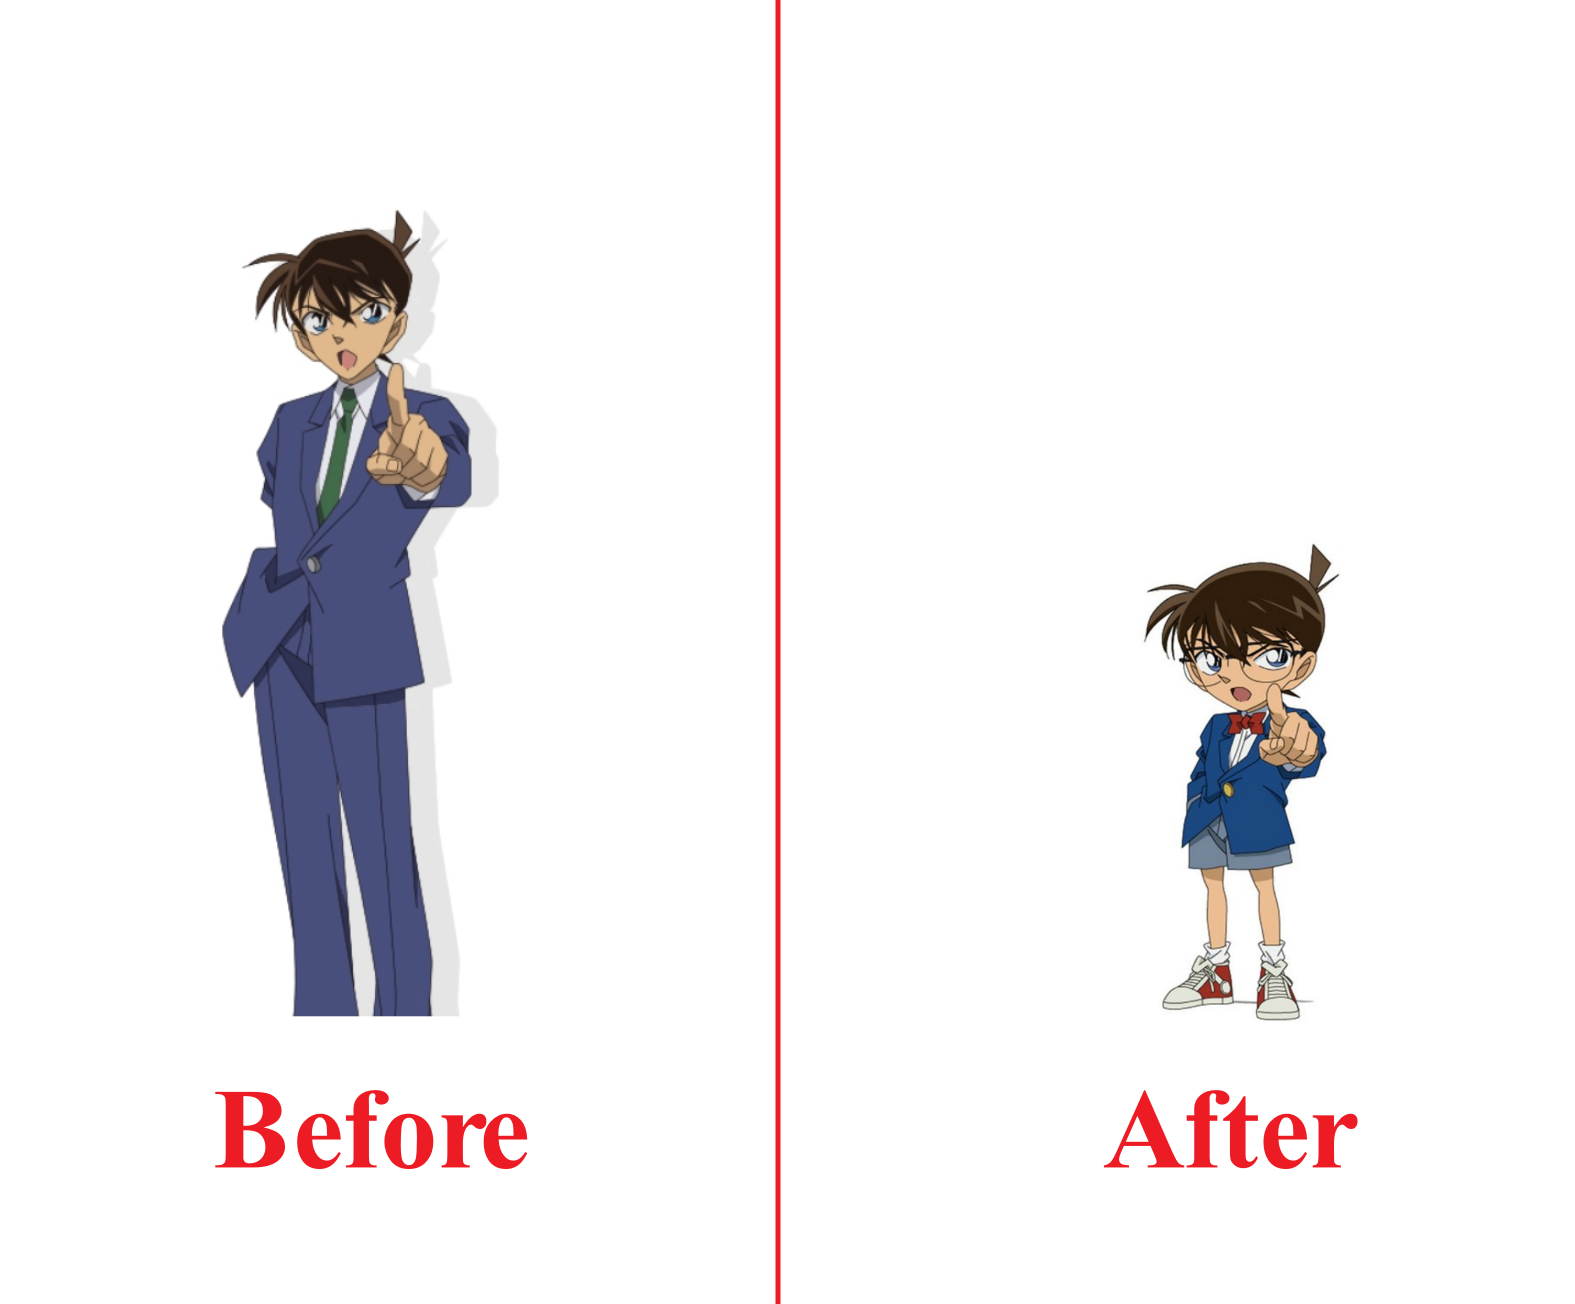
\includegraphics[width=\textwidth]{images/example_image_1.png}   
            \captionof{figure}{效果图。}
            \label{fig: example_1} 
        \end{minipage}
        \begin{minipage}[b]{0.32\linewidth}
            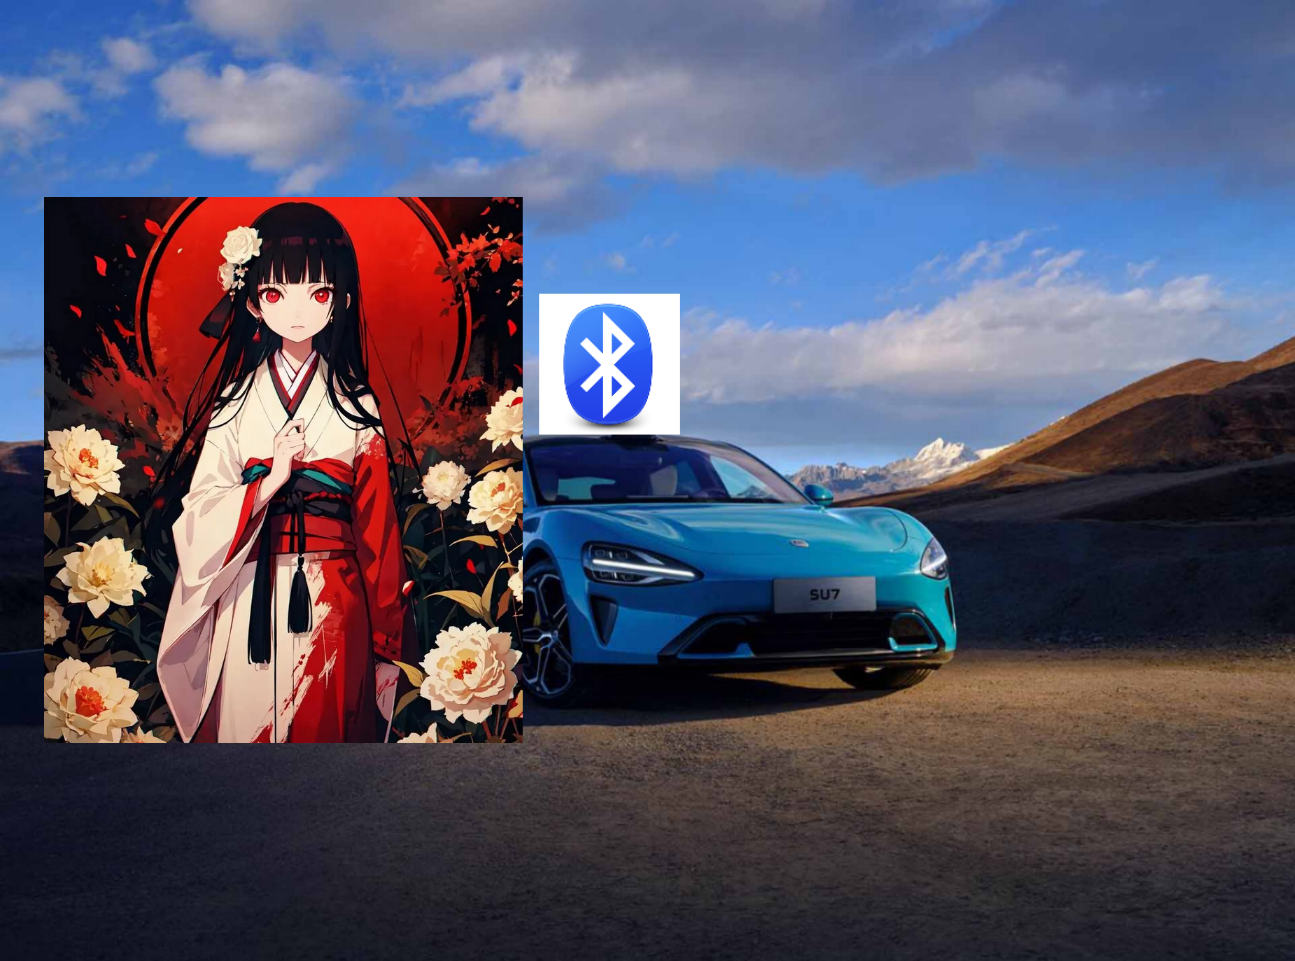
\includegraphics[width=\textwidth]{images/example_image_2.png}   
            \captionof{figure}{机器渲染图。}
            \label{fig: example_2} 
        \end{minipage}
        \begin{minipage}[b]{0.32\linewidth}
            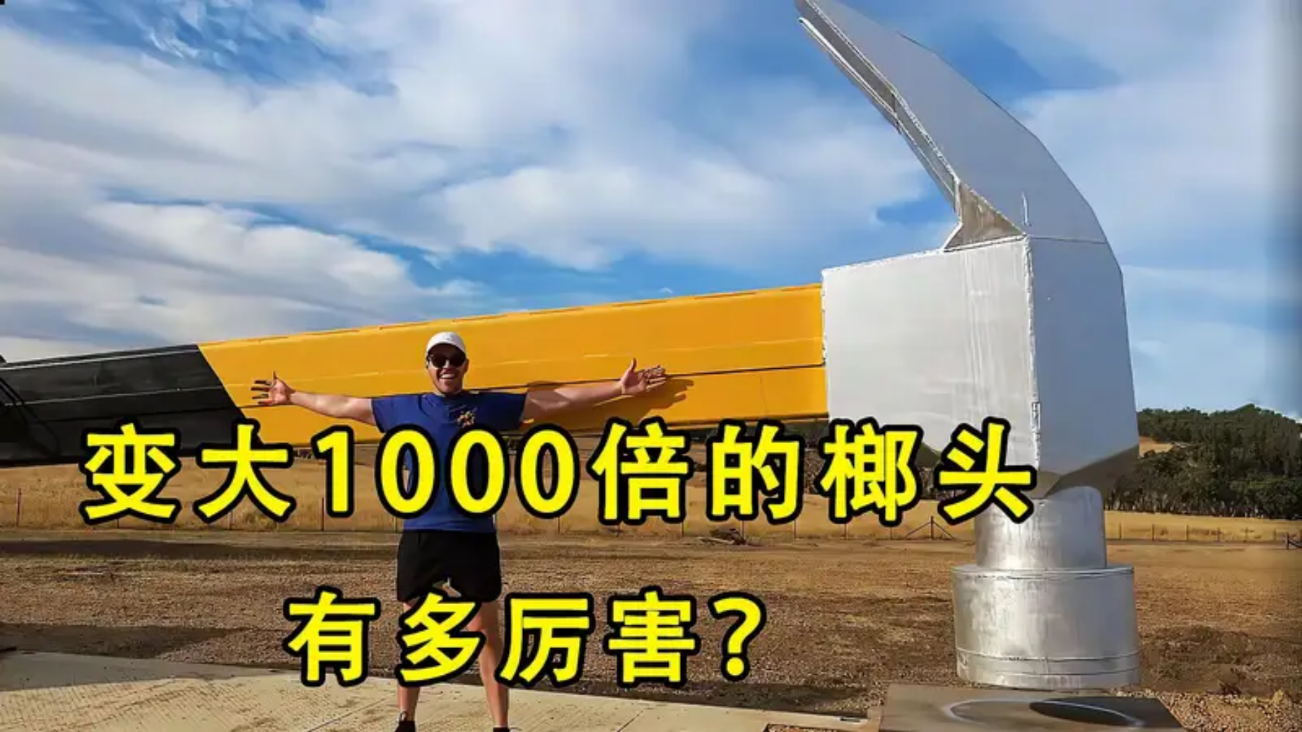
\includegraphics[width=\textwidth]{images/example_image_3.png}   
            \captionof{figure}{你看个锤子看。}
            \label{fig: example_3}
        \end{minipage}
    \end{figure}


    % 竞赛经历(找导师也可能看中这个,因为代表了一定实践能力,但是尽量对口吧,不要运动会都写进去了)
    \section{\makebox[\widthof{\faTrophy}][c]{\color{NPU_Blue}{\faTrophy}}\quad 竞赛经历}
    \vspace{-1em}           % table 前减一个1em会好看点
    \begin{table}[h!]
        \begin{tabularx}{\textwidth}{Xp{\widthof{第零负责人}}p{\widthof{国家级-第100名}}p{\widthof{2030年13月}}}
            \textbf{2023年全国大学生无聊透顶比赛} & 第一负责人 & 国家级-第10名 & 2023年4月 \\
            \textbf{2023年优质肛门大赛} & 个人参赛 & 国家级-一等奖 & 2023年8月\\
            \textbf{2022年全国大学生提肛大赛} & 个人参赛 & 省级-一等奖 & 2022年12月\\
            % 同理,可以自己加
        \end{tabularx}
    \end{table}

    {\LARGE \color{red}{或者你可以}}

    \begin{table}[h!]
        \begin{tabularx}{\textwidth}{Xp{\widthof{第零负责人}}p{\widthof{国家级-第100名}}p{\widthof{2030年13月}}}
            \textbf{2022年全国大学生交流大赛} & 技术负责人 & 省级-三等奖 & 2023年8月\\
        \end{tabularx}
    \end{table}
    \vspace{-1em}
    (“鸡同鸭讲”系统——一款全新的乱套翻译软件)主要负责了\textbf{移动端(安卓\&IOS)软件开发},\textbf{数据库建立与部署},实现了低达\textbf{0.01\%的翻译准确率}。

    \begin{table}[h!]
        \begin{tabularx}{\textwidth}{Xp{\widthof{第零负责人}}p{\widthof{国家级-第100名}}p{\widthof{2030年13月}}}
            \textbf{2022年全国大学生睡觉大赛} & 技术负责人 & 省级-一等奖 & 2023年4月\\
        \end{tabularx}
    \end{table}
    \vspace{-1em}
    (基于躺姿的标准8小时睡眠理论研究)主要负责了\textbf{躺姿的设计},枕头和床褥的选购。在队友的助眠协助下成功睡眠\textbf{8小时}。


    % 技能特长,上面写很多的话,这里就随便写点,反正上面都看出来了。上面写的不多的话,这里着重强调你会什么。
    % 哦,你找工作的话,这里多写点,记得对口,可以\textbf{}加粗。
    % 这里能吹牛皮就吹牛皮,但是确保面试的时候别露馅就行。
    \section{\makebox[\widthof{\faWrench}][c]{\color{NPU_Blue}{\faWrench}}\quad 技能特长}
    \vspace{0.5em}          % itemize 前加一个0.5em会好看点
    \begin{itemize}
        \item 熟练提肛技巧
        \item 在游戏中熟练使用C语言
        \item 熟悉安卓环境下的游戏安装
        \item 遇到困难会睡大觉
        \item 饿了会吃饭
        \item 尿急会上厕所
        \item 没钱了会让你发工资
    \end{itemize}


    % 换页
    \newnewpage


    % 所获荣誉(这个看你想不想写了)
    \section{\makebox[\widthof{\faStar}][c]{\color{NPU_Blue}{\faStar}}\quad 所获荣誉}
    \vspace{-1em}           % multicols 前减一个1em会好看点
    \begin{multicols}{2}
        \begin{itemize}
            \item 某年学业先进个人
            \item 某年某奖学金某等奖
            \item 某大使
            \item 某年某奖学金某等奖
            \item 某年优秀团员称号
            \item 某年某称号
        \end{itemize}
    \end{multicols}

    
    % 其他(也是看你想不想写)
    \section{\makebox[\widthof{\faInfo}][c]{\color{NPU_Blue}{\faInfo}}\quad 其他}
    \vspace{0.5em}          % itemize 前加一个0.5em会好看点
    \begin{itemize}
        \item 英语水平-CET6级xxx分
        \item 计算机几级证书
        \item xx几级证书
        \item 技术博客: 某网址
        \item 教师资格证:xxx
        \item 普通话证书:几级几等
        \item 文字排版:\LaTeX
    \end{itemize}
\end{document}
%%%%%%%%%%%%%%%%%%%%%%%%%%%%%%%%%%%%%%%%%%%%%%%%%%%%%%%%%%%%%%%%%
%							正文结束							%
%%%%%%%%%%%%%%%%%%%%%%%%%%%%%%%%%%%%%%%%%%%%%%%%%%%%%%%%%%%%%%%%%
